%%%%%%%%%%%%%%%%%%%%%%%%%%%%%%%%%%%%%%%%%
% NIWeek 2014 Poster by T. Reveyrand
% www.microwave.fr
% http://www.microwave.fr/LaTeX.html
% ---------------------------------------
%
% Original template created by:
% Brian Amberg (baposter@brian-amberg.de)
%
% This template has been downloaded from:
% http://www.LaTeXTemplates.com
%
% License:
% CC BY-NC-SA 3.0 (http://creativecommons.org/licenses/by-nc-sa/3.0/)
%
%%%%%%%%%%%%%%%%%%%%%%%%%%%%%%%%%%%%%%%%%

%----------------------------------------------------------------------------------------
%	PACKAGES AND OTHER DOCUMENT CONFIGURATIONS
%----------------------------------------------------------------------------------------

\documentclass[a0paper,portrait]{baposter}

\usepackage[font=small,labelfont=bf]{caption} % Required for specifying captions to tables and figures
\usepackage{booktabs} % Horizontal rules in tables
\usepackage{relsize} % Used for making text smaller in some places

\usepackage{amsmath, amsfonts, amssymb, amsthm} % Math packages
\usepackage{eqparbox}
\usepackage{boldline, multirow}

\usepackage{textcomp}

\usepackage{hyperref}

\graphicspath{{images/}} % Directory in which figures are stored

 \definecolor{bordercol}{RGB}{40,40,40} % Border color of content boxes
 \definecolor{headercol1}{RGB}{186,215,230} % Background color for the header in the content boxes (left side)
 \definecolor{headercol2}{RGB}{120,120,120} % Background color for the header in the content boxes (right side)
 \definecolor{headerfontcol}{RGB}{0,0,0} % Text color for the header text in the content boxes
 \definecolor{boxcolor}{RGB}{210,235,250} % Background color for the content in the content boxes

\definecolor{jdhblue}{RGB}{2,93,186}

\definecolor{zkblue}{RGB}{88,135,175}
\definecolor{zkbackground}{RGB}{230,232,234}


\usetikzlibrary{shapes, arrows, external, decorations.pathmorphing, backgrounds, positioning, fit, petri, calc, hobby, cd}


\begin{document}

% \background{ % Set the background to an image (background.pdf)
% \begin{tikzpicture}[remember picture,overlay]
% \draw (current page.north west)+(-2em,2em) node[anchor=north west]
% {\includegraphics[height=1.1\textheight]{images/baposter_background.pdf}};
% \end{tikzpicture}
% }

\begin{poster}{
grid=false,
borderColor=bordercol, % Border color of content boxes
headerColorOne=headercol1, % Background color for the header in the content boxes (left side)
headerColorTwo=headercol2, % Background color for the header in the content boxes (right side)
headerFontColor=headerfontcol, % Text color for the header text in the content boxes
% boxColorOne=boxcolor, % Background color for the content in the content boxes
boxColorOne=zkbackground,
headershape=roundedright, % Specify the rounded corner in the content box headers
headerfont=\Large\sf\bf, % Font modifiers for the text in the content box headers
textborder=rectangle,
% background=user,
background=none,
headerborder=open, % Change to closed for a line under the content box headers
boxshade=plain
}
%
%----------------------------------------------------------------------------------------
%	TITLE AND AUTHOR NAME
%----------------------------------------------------------------------------------------
%
{
\includegraphics[scale=0.101]{logo_tmu.jpeg}} % University/lab logo
{
{\bf \fontsize{19pt}{19pt} \selectfont Predicting Neurological Recovery from Coma with Longitudinal EEG Using Deep Neural Networks}
} % Poster title
{\vspace{0.3em} \smaller Jingsu KANG$^1$, Hao WEN$^2$  \\  % Author names

$^1${\it Tianjin Medical University}\qquad
$^2${\it College of Science, China Agricultural University} \\
\vspace{0.2cm}
{\Large \bf{The George B. Moody PhysioNet Challenge 2023}, ~~~\bf{Team Revenger}}
}
{
\includegraphics[scale=0.401]{images/logo_cau_science.png}}


\newif\ifcoloredtext
\coloredtexttrue
\newif\ifboxednn
\boxednntrue


%----------------------------------------------------------------------------------------
%	INTRODUCTION
%----------------------------------------------------------------------------------------

\headerbox{Introduction}{name=introduction, column=0, row=0, span=3}{
% finished

\begin{itemize}
\item We modeled the problem as a \textbf{classification problem} where the learning objective is the discrete CPC scores (1 - 5). The final clinical outcome prediction is obtained via the mapping: CPC = 1 or 2 $\to$ ``Good outcome''; CPC = 3, 4, or 5 $\to$ ``Poor outcome''.
\vspace{-0.2cm}
\item Offline signal quality index (SQI) was computed offline for EEG recordings. A part of EEGs was selected for training based on SQI.
\vspace{-0.2cm}
\item We used a \textbf{time-incremental convolutional recurrent neural network (TiCRNN model} to make per-recording probability vectors, which were averaged and re-normalized via \texttt{Softmax} to obtain per-patient predictions from multiple EEG recordings.
\end{itemize}
}


%----------------------------------------------------------------------------------------
%	NN architecture
%----------------------------------------------------------------------------------------

\headerbox{Main Model: TiCRNN}{name=nn, column=0, span=1, row=1, below=introduction}{
% finished

% \input{plot_figures/model_arch}

% \vspace{-0.3cm}

We used a {\color{red}T}ime-{\color{red}i}ncremental {\color{red}C}onvolutional {\color{red}R}ecurrent {\color{red}N}eural {\color{red}N}etwork ({\color{red}TiCRNN}) model to predict probabilities of CPC scores for the EEG recordings. Multiple results from one patient were merged via averaging and softmax.
}

%----------------------------------------------------------------------------------------
%	NN Backbone
%----------------------------------------------------------------------------------------

\headerbox{Neural Network Backbone}{name=backbone, column=1, span=2, row=1, below=introduction}{
% finished

% \input{plot_figures/se_bottleneck}%
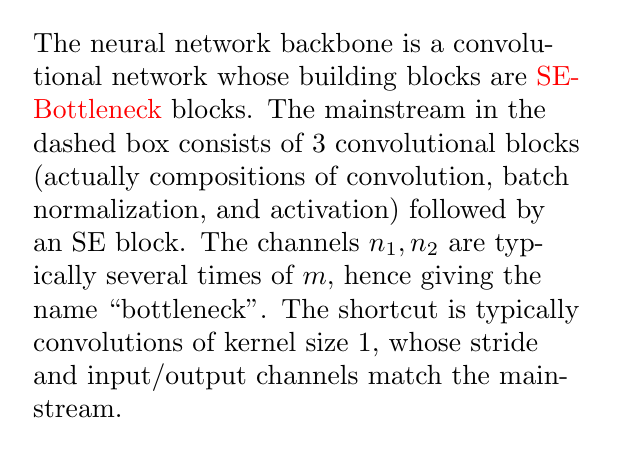
\begin{tikzpicture}
\node [rectangle, text width = 20em, inner sep = 2pt, minimum height = 1.0em] {The neural network backbone is a convolutional network whose building blocks are {\color{red}SE-Bottleneck} blocks. The mainstream in the dashed box consists of 3 convolutional blocks (actually compositions of convolution, batch normalization, and activation) followed by an SE block. The channels $n_1, n_2$ are typically several times of $m,$ hence giving the name ``bottleneck''. The shortcut is typically convolutions of kernel size 1, whose stride and input/output channels match the mainstream.};
\end{tikzpicture}

}

%----------------------------------------------------------------------------------------
%	Preprocessing
%----------------------------------------------------------------------------------------

\headerbox{Preprocess Pipeline}{name=data, column=2, row=1, span=1, below=backbone}{
% finished

\begin{itemize}
\item Select at most one 5-minute window from each recording by offline-computed SQI.
\vspace{-0.2cm}
\item Butterworth bandpass filtering of order 4 and cutoff frequencies 0.5 - 30 Hz.
\vspace{-0.2cm}
\item Resampling to 100 Hz using polyphase filtering.
\vspace{-0.2cm}
\item Rescaling (Z-score normalization) to zero mean and unit variance.
\end{itemize}
}

%----------------------------------------------------------------------------------------
%	Training Setups
%----------------------------------------------------------------------------------------

\headerbox{Training Strategies}{name=training, span=1, column=1, row=1, below=backbone}{
% finished

\begin{itemize}
\item Optimizer: AMSGrad variant of AdamW with OneCycleLR scheduler.
\vspace{-0.2cm}
\item Stratified train-validation split (split among patients): 80 \% -- 20 \%.
\vspace{-0.2cm}
\item Batch size 32; epoch number $\leq 55$ with early stopping patience 25 epochs.
\vspace{-0.2cm}
\item Input length 180s, randomly sliced from one recording and reloads every 5 epochs.
\end{itemize}
}

%----------------------------------------------------------------------------------------
%	Importance of Rescaling
%----------------------------------------------------------------------------------------

\headerbox{Importance of Rescaling}{name=rescale, span=1, column=2, below=data}{
% finished

% \includegraphics[width=\linewidth]{images/train_scores_compare.pdf}

Mean curves of challenge scores on the training set. Shaded areas are error bounds.

}

%----------------------------------------------------------------------------------------
%	Submission Results
%----------------------------------------------------------------------------------------

\headerbox{Submission Results}{name=submission, span=2, column=0, below=training}{
% almost finished
% TODO: update the scores on the training and cross-val sets

\renewcommand{\arraystretch}{1.25}
\begin{center}
% requires packages boldline, multirow
\setlength\tabcolsep{4pt}
% \begin{tabular}{@{\extracolsep{6pt}}c|c|c|c|c@{}}
\begin{tabular}{c|c|c|c|c}
\hlineB{3.5}
& \multicolumn{4}{c}{\textbf{Challenge Scores}} \\ \cline{2-5}
& \textbf{72 hours} & 12 hours & 24 hours & 48 hours \\ \hline
Training & 0.814 $\pm$ 0.070 & - & - & - \\
Cross-validation & 0.424 $\pm$ 0.026 & - & - & - \\ \hline
Hidden validation & \textbf{0.701} & 0.33 & 0.40 & \textbf{0.75} \\
Ranking & \textbf{5 / 270} & - & - & - \\
\hlineB{3.5}
\end{tabular}
\end{center}
\renewcommand{\arraystretch}{1}

\begin{itemize}
\item Challenge score and ranking evaluated on the hidden validation set, scores on its truncated 12h / 24h / 48h subsets, and scores on the training and cross-validation sets.
\vspace{-0.2cm}
\item Scores on the train and cross-validation sets are of the form $mean \pm std. dev.$ from all our offline experiments with z-score normalization included in the preprocessing pipeline.
\end{itemize}

}

%----------------------------------------------------------------------------------------
%	Limitations, Discussions
%----------------------------------------------------------------------------------------

\headerbox{Discussions and Limitations}{name=discussion, column=0, below=submission, span=3}{
% almost finished

\begin{itemize}
\item Our team provided a solution that is relatively simple and lightweight, but still able to attain a TPR as high as 0.701 with FPR suppressed to a very low level ($\le 0.05$) for poor clinical outcome prediction.
\vspace{-0.2cm}
\item Our team made too much trade-off for the limited computation resources by dropping a large proportion of the EEG data by SQI thresholding and random slicing. The data amount (counting by time length) we really used for training the NN models merely constitutes 6 \% of the total EEG data. The potential of this extraordinarily big data had not yet been fully explored.
\vspace{-0.2cm}
\item Our team had planned to make full use of the data to train a larger model that learns latent representations from EEGs via unsupervised contrastive learning. However, due to the constraints of time and computation resources our team owns, we finally decided to stick to the simpler TiCRNN model. Architecture design and unsupervised training mechanisms for large EEG models are left as future research directions.
\vspace{-0.2cm}
\item The computation of SQI for EEGs is time-consuming. This prohibited us from adding a similar selection procedure in the pipeline of model evaluation on the hidden data and is highly probable to have a negative influence on our overall performance, especially for EEGs heavily contaminated with artifacts. Therefore, developing a faster and end-to-end SQI computation method would also be a meaningful research problem.
\end{itemize}

}


%----------------------------------------------------------------------------------------
%	REFERENCES
%----------------------------------------------------------------------------------------

% \headerbox{References}{name=references,column=2,below=application}{

% \smaller % Reduce the font size in this block
% \renewcommand{\section}[2]{\vskip 0.05em} % Get rid of the default "References" section title
% \nocite{*} % Insert publications even if they are not cited in the poster

% \bibliographystyle{unsrt}
% \bibliographystyle{IEEEtran}
% \bibliography{biblio} % Use biblio.bib as the bibliography file
% }


%----------------------------------------------------------------------------------------
%	ACKNOWLEDGEMENTS
%----------------------------------------------------------------------------------------

\headerbox{Acknowledgements}{name=acknowledgements, column=0, below=discussion, span=3}{
% finished
% \smaller
We would like to thank professor {\bf Deren Han} from the School of Mathematical Sciences, Beihang University and professor {\bf Wenjian Yu} from the Department of Computer Science and Technology, BNRist, Tsinghua University for generously providing GPU servers to help accomplish this work.

}

%----------------------------------------------------------------------------------------
%	link to the GitHub repository
%----------------------------------------------------------------------------------------

\headerbox{}{name=foottext, column=0, span=3, below=acknowledgements, textborder=none, headerborder=none,  boxheaderheight=0pt}{
% finished
\hfill \small \textit{Code, configs, etc. available at https://github.com/DeepPSP/cinc2023, and based on https://github.com/DeepPSP/torch\_ecg.}
}


\end{poster}

\end{document}
